\documentclass[11pt,a4paper]{article}
\usepackage[T1]{fontenc}\usepackage{lmodern}\usepackage[margin=2.2cm]{geometry}\usepackage{microtype}
\usepackage{booktabs}\usepackage{tabularx}\usepackage{array}\usepackage{float}\usepackage{multirow}
\usepackage{caption}\usepackage{enumitem}\usepackage{xcolor}\usepackage{amsmath}\usepackage{pdflscape}
\usepackage{tikz}\usetikzlibrary{positioning,arrows.meta,fit,backgrounds,calc,shapes.geometric}
\usepackage{tcolorbox}
\usepackage[colorlinks=true,linkcolor=blue!50!black,urlcolor=blue!50!black,citecolor=blue!50!black]{hyperref}
\captionsetup{font=small,labelfont=bf}\setlist{itemsep=2pt,topsep=3pt}\setlength{\emergencystretch}{3em}
\newcolumntype{Y}{>{\raggedright\arraybackslash}X}
\newtcolorbox{keybox}[1]{colback=blue!3,colframe=blue!45!black,title=#1,fonttitle=\bfseries,sharp corners,boxrule=0.6pt}
\newtcolorbox{onesentence}{colback=gray!6,colframe=gray!50,sharp corners,boxrule=0.4pt,left=4pt,right=4pt,top=2pt,bottom=2pt}
\newcommand{\say}[1]{\begin{onesentence}\small\textbf{In one sentence:} #1\end{onesentence}}
\newcommand{\why}[1]{\par\noindent\textit{Why:} #1\par}
\definecolor{cSrc}{HTML}{E8E8E8}\definecolor{cPrep}{HTML}{DCE9F7}\definecolor{cGen}{HTML}{FCE5CD}
\definecolor{cFeat}{HTML}{D9EAD3}\definecolor{cModel}{HTML}{E4DCF2}\definecolor{cOut}{HTML}{F4CCCC}
\definecolor{cEval}{HTML}{FFF2CC}

\title{\vspace{-1cm}\textbf{Robust Video Source Provenance: Distinguishing Synthetic vs.\ Organic Sensor Noise to Counter Anti-Forensic Injection Attacks}\\[8pt]
\large Mid-Evaluation Report --- the Hybrid Video Provenance Framework (HVPF)}
\author{Talha Aslam\\[2pt] \small Supervisor: Dr.\ Hasan Mujtaba \quad Co-supervisor: Dr.\ Muhammad Ishtiaq\\
\small Department of Artificial Intelligence \& Data Science, FAST-NUCES Islamabad}
\date{20 October 2026}

\begin{document}
\maketitle

\begin{keybox}{At a glance: what to tell the panel}
\begin{itemize}[leftmargin=12pt]
\item \textbf{Problem.} A camera's sensor leaves a fingerprint in every video (PRNU). Forensic tools use it to verify where a
      video came from. Attackers can \emph{remove} that fingerprint, \emph{forge} another camera's fingerprint, or generate the
      whole video with AI and then inject a real camera's fingerprint into it.
\item \textbf{What I built.} HVPF, a pipeline that decides for every video clip whether it is \emph{organic} (genuine camera
      footage), \emph{manipulated} (an anti-forensic attack on the fingerprint) or \emph{synthetic} (AI-generated), by combining
      PRNU analysis with machine learning and deep learning (a Vision Transformer).
\item \textbf{Data.} Three real-camera datasets (VISION, Video-ACID, FloreView; 124 usable cameras), eight AI generators for
      training and four unseen ones for testing; 46,799 clips in the current phase.
\item \textbf{Main result so far (Phase 3).} On cameras never seen in training, the hybrid model reaches macro F1 0.851 and
      AUC 0.941 for genuine vs.\ not genuine; the conventional PRNU method reaches AUC 0.549. AI videos with an injected camera
      fingerprint pass the conventional check 98\% of the time, but the hybrid model only 0--1\%.
\item \textbf{Honest evaluation.} Three ``shortcuts'' that inflate scores were found and removed (WhatsApp compression,
      clip length, encoder traces). Results are reported on unseen camera models, unseen phones (FloreView) and unseen AI generators.
\item \textbf{Now running (Phase 4).} Attacks on a second dataset, four more AI generators, more genuine platform copies, a
      10-frame ViT and a ``safe'' decision rule. Trained camera identification is already done: 94.9\% on Video-ACID.
\end{itemize}
\end{keybox}

\tableofcontents
\newpage

%=====================================================================================================
\section{Introduction}

\subsection{The problem in plain words}
Every camera sensor has tiny, permanent differences in how sensitive each pixel is to light. These differences leave a faint
pattern, the \emph{Photo-Response Non-Uniformity} (PRNU), in every image and video the camera records. Because the pattern
is unique to one sensor, it works like a fingerprint: by comparing the noise in a video with a camera's fingerprint, an
analyst can verify whether that camera recorded the video. Courts and investigators rely on this.

The problem is that the fingerprint can be attacked:
\begin{itemize}
\item \textbf{Removal}: an attacker subtracts the camera's fingerprint, so the video can no longer be traced to its source.
\item \textbf{Injection (transfer)}: an attacker adds \emph{another} camera's fingerprint, so the video appears to come from
      that camera (Khan et al.\ 2025 show this fools verification for 85.5\% of images).
\item \textbf{AI generation}: a video made by a generator (Sora, Kling, \dots) has no camera at all; an attacker can still
      inject a real camera's fingerprint into it, so it passes as genuine footage of that camera.
\item \textbf{Everyday processing}: re-compression by WhatsApp or YouTube, resizing and video stabilisation weaken the
      fingerprint even without any attack.
\end{itemize}
The conventional method (a correlation score called PCE above a threshold) only asks ``is this camera's fingerprint present?''.
It cannot tell genuine sensor noise from noise that was added or synthesised. This thesis builds a system that can.

\subsection{Research gaps (from the thesis proposal)}
\begin{enumerate}[label=\textbf{Gap \arabic*:},leftmargin=45pt]
\item Existing methods \emph{link} media to a camera but do not decide whether the sensor noise itself is genuine or artificial.
\item Most work is on still images; video adds compression, transcoding and stabilisation, and adversarial video settings are
      rarely tested.
\item Source attribution and synthetic-media detection are studied separately; few frameworks combine PRNU analysis, machine
      learning and deep learning in one system.
\end{enumerate}

\subsection{Research questions and where they are answered}
\begin{table}[H]\centering\small
\begin{tabularx}{\linewidth}{lYl}\toprule
& Research question & Answered by \\\midrule
RQ1 & What discriminative characteristics differentiate organic sensor noise from synthetic or manipulated noise? &
      Feature ablation (Sec.~\ref{sec:rq1}) \\
RQ2 & How do compression, resizing, filtering and frame manipulation affect PRNU-based attribution and noise-based analysis? &
      Per-condition results (Sec.~\ref{sec:rq2}), Step 4 \\
RQ3 & Can a hybrid PRNU + ML/DL framework improve accuracy and robustness over conventional forensic methods? &
      Hybrid vs.\ PCE rule (Sec.~\ref{sec:rq3}), Step 10 \\\bottomrule
\end{tabularx}\end{table}
The six objectives of the proposal map onto the pipeline as follows: analysing PRNU in genuine video (Steps 3--4), studying
how attacks alter it (Steps 5--6), finding discriminative features (Step 7, ablation), building the hybrid framework
(Steps 8--8c, 10), testing robustness (Step 9, all conditions) and improving real-world reliability (unseen cameras,
unseen generators, safe operating point).

\subsection{Contributions so far}
\begin{enumerate}
\item A three-class provenance framework (organic / manipulated / synthetic) for \emph{video} that combines PRNU, Noiseprint++,
      noise statistics, temporal noise consistency and a Vision Transformer.
\item The first evaluation (to our knowledge) of PRNU transfer attacks on video, including PRNU injected into
      AI-generated video, against both the conventional method and the hybrid detector.
\item An evaluation protocol designed against leakage and shortcuts: camera-model-grouped splits, unseen cameras and
      generators, an encoder-controlled setting, and a documented analysis of three shortcuts.
\item Trained source camera identification combined with PRNU (a hybrid), which works on stabilised phones where PRNU fails.
\item Open, reproducible code: \url{https://github.com/TalhaAslam44/PRNU-Research}.
\end{enumerate}

%=====================================================================================================
\section{Background concepts}\label{sec:background}
\begin{description}[leftmargin=0pt]
\item[Noise residual $W$.] The image $I$ minus a denoised version of itself, $W = I - F(I)$. It keeps the fine noise
      (including PRNU) and removes most of the scene.
\item[PRNU fingerprint $K$.] Estimated from many frames of one camera with the maximum-likelihood estimator
      $K = \sum_i W_i I_i / \sum_i I_i^2$ (Polimi \texttt{prnu-python}). The sensor output is approximately $I \approx I^{(0)}(1+K)$.
\item[NCC and PCE.] To test whether a video comes from camera $c$, the residual of the video is correlated with $I \cdot K_c$.
      NCC is the normalised correlation; PCE (peak-to-correlation energy) measures how far the correlation peak stands above
      the rest of the correlation surface. PCE$_0$ is PCE at zero shift (frames are already aligned).
      \textbf{Conventional rule: PCE$_0 > 60$ means ``recorded by this camera''.}
\item[I-frames.] Video codecs store a few complete frames (I-frames) and many predicted frames between them. I-frames keep
      the most sensor noise, so all analysis uses I-frames.
\item[Noiseprint++.] A neural network (GRIP, TruFor) that extracts a camera-model fingerprint and suppresses scene content.
      We use statistics of its output.
\item[TSNCS.] Temporal sensor-noise consistency: the correlation between the noise residuals of consecutive frames. Genuine
      noise behaves consistently over time; strong removal and AI generation disturb it.
\item[SRM filters.] Fixed high-pass filters from steganalysis that turn an image into noise residuals. The Vision Transformer
      sees these residuals, not the scene.
\item[Vision Transformer (ViT).] A deep network that cuts an image into $16\times16$ patches and models relations between
      them with attention. We fine-tune ViT-S/16 (21.7M parameters) pretrained on ImageNet-21k.
\end{description}

%=====================================================================================================
\section{System architecture}\label{sec:arch}
Figure~\ref{fig:arch} shows the complete framework. It has six stages, read from left to right: data sources; preparation
(Steps 1--3); reference and test material (Steps 4--6); forensic evidence (Step 7); learning (Steps 8 and 8b); and fusion,
decision and evaluation (Steps 8c and 9). A separate branch (Step 10) answers the classic forensic question ``which camera
recorded this video?''. Figure~\ref{fig:detector} zooms into the hybrid detector itself.

\begin{landscape}
\begin{figure}
\centering
\begin{tikzpicture}[
  font=\scriptsize, >={Stealth[length=2.2mm]},
  box/.style={draw=black!55, rounded corners=2pt, align=left, text width=3.35cm, inner sep=3pt, line width=0.5pt},
  src/.style={box, fill=cSrc}, prep/.style={box, fill=cPrep}, gen/.style={box, fill=cGen},
  feat/.style={box, fill=cFeat}, model/.style={box, fill=cModel}, decide/.style={box, fill=cOut}, eval/.style={box, fill=cEval},
  head/.style={font=\footnotesize\bfseries, text width=3.6cm, align=center},
  arr/.style={->, draw=black!70, line width=0.6pt}, bus/.style={draw=black!70, line width=0.6pt}]
% column headers
\node[head] at (0,1.55) {Data sources};
\node[head] at (4.3,1.55) {Preparation\\(Steps 1--3)};
\node[head] at (8.6,1.55) {Reference \& test material\\(Steps 4--6)};
\node[head] at (12.9,1.55) {Forensic evidence\\(Step 7)};
\node[head] at (17.2,1.55) {Learning\\(Steps 8, 8b)};
\node[head] at (21.5,1.55) {Fusion, decision, evaluation\\(Steps 8c, 9)};
% data sources
\node[src] (vis) at (0,0) {\textbf{VISION}\\35 cameras; native, real YouTube and WhatsApp copies};
\node[src] (acid) at (0,-2.05) {\textbf{Video-ACID}\\44 cameras, 200 videos each};
\node[src] (fv) at (0,-4.1) {\textbf{FloreView}\\45 modern phones\\\textit{unseen: test only}};
\node[src] (gvb) at (0,-6.15) {\textbf{GenVidBench}\\8 AI generators (Sora, Kling, CogVideo, OpenSora, SVD, Mora, T2V-Zero, Pika)};
\node[src] (gb) at (0,-8.3) {\textbf{GenBuster}\\4 AI generators\\\textit{unseen: test only}};
\begin{scope}[on background layer]\node[draw=black!40, dashed, rounded corners, fit=(vis)(gb), inner sep=4pt] (srcbox) {};\end{scope}
% preparation
\node[prep] (s1) at (4.3,0) {\textbf{Step 1 -- Inventory}\\ffprobe every video: codec, resolution, rotation, I-frames, bitrate};
\node[prep] (s2) at (4.3,-2.6) {\textbf{Step 2 -- Splits}\\grouped by \emph{camera model}: train / val / test (60/20/20) + 5 folds; reference vs.\ sample videos};
\node[prep] (s3) at (4.3,-5.3) {\textbf{Step 3 -- I-frames}\\up to 30 I-frames per video, $480\times480$ luma crop; rotation and platform rescaling undone};
\draw[arr] (srcbox.east |- s1) -- (s1);
\draw[arr] (s1) -- (s2); \draw[arr] (s2) -- (s3);
% reference & test material
\node[gen] (s4) at (8.6,0) {\textbf{Step 4 -- PRNU fingerprints}\\$K$ per camera from reference videos; PCE / NCC attribution baseline};
\node[gen] (org) at (8.6,-2.6) {\textbf{Genuine clips} (organic)\\natural videos, real platform copies, genuine re-encodes + their platform copies};
\node[gen] (s5) at (8.6,-5.2) {\textbf{Step 5 -- Manipulated}\\PRNU removal, PRNU injection, denoising; WhatsApp-/YouTube-like copies; VISION + ACID};
\node[gen] (s6) at (8.6,-7.85) {\textbf{Step 6 -- Synthetic}\\AI clips re-encoded like the rest; claimed camera; Khan-style PRNU injection; platform copies};
\draw[bus] (s3.east) -- (6.55,-5.3);
\draw[bus] (6.55,0) -- (6.55,-7.85);
\foreach \n in {s4,org,s5,s6} \draw[arr] (6.55,0 |- \n) -- (\n.west);
\node[font=\tiny, rotate=90, fill=white, inner sep=1pt] at (6.55,-6.55) {videos, frames, splits};
% forensic evidence
\node[feat, text width=3.45cm] (s7) at (12.9,-2.55) {\textbf{Step 7 / 7b -- Features}\\
  \textbullet\ PRNU: NCC, PCE$_0$ vs.\ claimed camera and best \emph{other} camera\\
  \textbullet\ residual statistics\\ \textbullet\ FFT statistics\\ \textbullet\ TSNCS (temporal consistency)\\
  \textbullet\ Noiseprint++ statistics (7b)\\ per frame and per clip};
\node[feat] (store) at (12.9,-6.6) {\textbf{Frame store}\\first 5 (or 10) I-frames of every clip; 46,799 clips (Phase 4)};
\draw[bus] (org.east) -- (10.95,-2.6); \draw[bus] (s5.east) -- (10.95,-5.2); \draw[bus] (s6.east) -- (10.95,-7.85);
\draw[bus] (10.95,-2.6) -- (10.95,-7.85);
\draw[arr] (10.95,-6.6) -- (store.west);
\draw[arr] (s4.east) -| (s7.north) node[pos=0.3, above, font=\tiny] {fingerprints $K$};
\draw[arr] (store) -- (s7);
% learning
\node[model] (base) at (17.2,0.1) {\textbf{Baseline}: conventional PCE rule\\PCE$_0$(claimed camera) $>60$ $\Rightarrow$ genuine};
\node[model] (cls) at (17.2,-2.0) {\textbf{Classical ML}\\SVM, XGBoost on clip features};
\node[model] (seq) at (17.2,-4.15) {\textbf{Sequence models}\\GRU, 1D-CNN, Transformer on frame sequences + clip features};
\node[model] (vit) at (17.2,-6.6) {\textbf{Step 8b -- ViT-S/16}\\on SRM noise residuals of the I-frames};
\draw[bus] (s7.east) -- (15.15,-2.55); \draw[bus] (15.15,0.1) -- (15.15,-4.15);
\foreach \n in {base,cls,seq} \draw[arr] (15.15,0 |- \n) -- (\n.west);
\draw[arr] (store.east) -- (vit.west);
% fusion, decision, evaluation
\node[decide] (fus) at (21.5,-2.0) {\textbf{Step 8c -- Fusion}\\calibration, ensembles, \textbf{stacking} (fitted on validation cameras), safe operating point};
\node[decide, fill=cOut!70!red!35] (dec) at (21.5,-4.6) {\textbf{Decision per clip}\\organic / manipulated / synthetic\\+ genuine-vs-not score};
\node[eval] (s9) at (21.5,-7.2) {\textbf{Step 9 -- Evaluation}\\PVA, macro-F1, AUC, EER, per condition, ablation, unseen sources, low-FPR, compromise rate};
\draw[bus] (cls.east) -- (19.35,-2.0); \draw[bus] (seq.east) -- (19.35,-4.15); \draw[bus] (vit.east) -- (19.35,-6.6);
\draw[bus] (19.35,-2.0) -- (19.35,-6.6); \draw[arr] (19.35,-2.0) -- (fus.west);
\draw[arr, dashed] (base.east) -| (21.5,-1.15) node[pos=0.25, above, font=\tiny] {compared};
\draw[arr] (fus) -- (dec); \draw[arr] (dec) -- (s9);
% step 10
\node[eval, fill=cPrep!60, text width=7.6cm] (s10) at (15.0,-9.55) {\textbf{Step 10 -- Camera identification by training}\\
  ViT with one output per camera (80/20 per camera, scene-grouped) + PRNU matching (Step 4) $\Rightarrow$ \textbf{hybrid}: PRNU
  when it is confident, otherwise the ViT};
\node[decide] (cam) at (21.5,-9.55) {\textbf{Which camera?}\\VISION 67.4\%, ACID 94.9\%, FloreView 90.1\%};
\draw[arr] (store.south) -- (store.south |- s10.north);
\draw[arr] (s10) -- (cam);
\end{tikzpicture}
\caption{Complete architecture of the Hybrid Video Provenance Framework (HVPF). Grey: data; blue: preparation; orange:
reference and test material; green: forensic evidence; purple: learning; red: fusion and decision; yellow: evaluation.
The conventional PCE rule (dashed) is the baseline every model is compared with.}\label{fig:arch}
\end{figure}
\end{landscape}

\begin{figure}[H]\centering
\resizebox{\linewidth}{!}{%
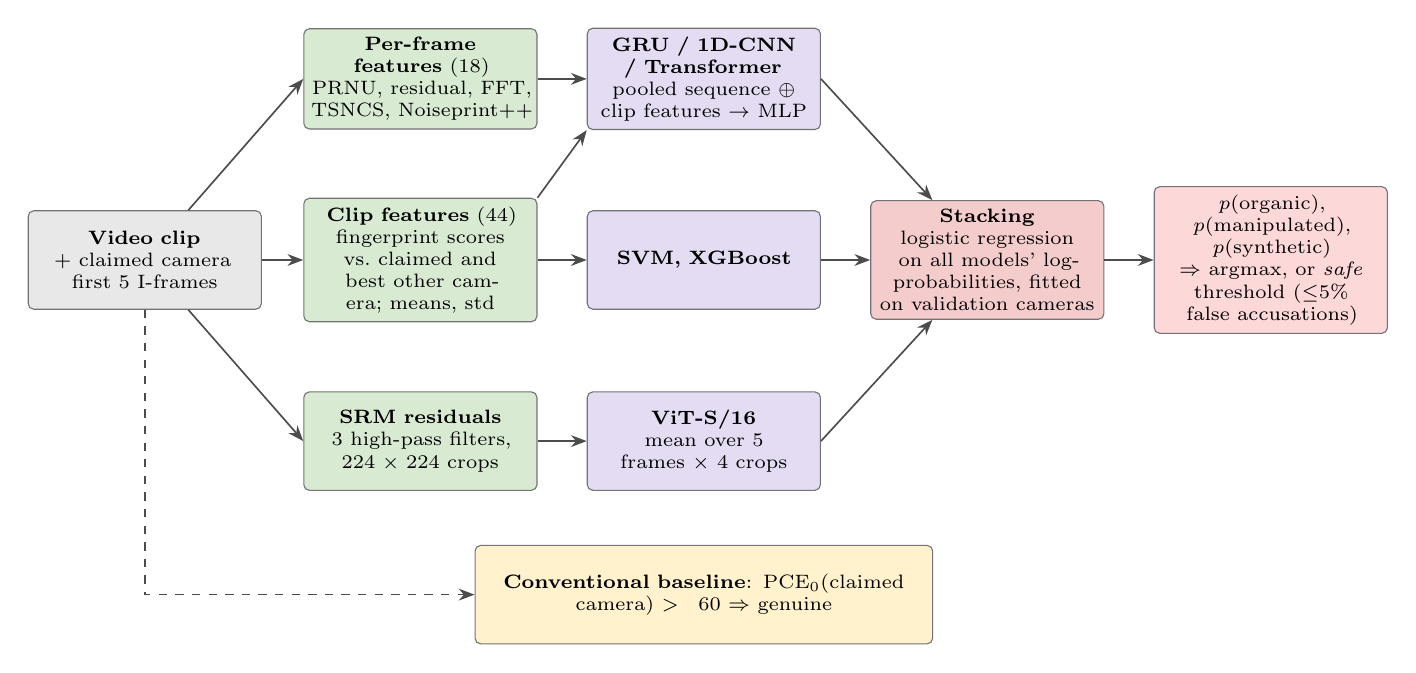
\begin{tikzpicture}[font=\scriptsize, >={Stealth[length=2mm]},
  box/.style={draw=black!55, rounded corners=2pt, align=center, text width=2.75cm, inner sep=3pt, minimum height=1.25cm},
  arr/.style={->, draw=black!70, line width=0.6pt}]
\node[box, fill=cSrc] (in) at (0,0) {\textbf{Video clip}\\+ claimed camera\\first 5 I-frames};
\node[box, fill=cFeat] (fa) at (3.5,2.3) {\textbf{Per-frame features} (18)\\PRNU, residual, FFT, TSNCS, Noiseprint++};
\node[box, fill=cFeat] (fb) at (3.5,0) {\textbf{Clip features} (44)\\fingerprint scores vs.\ claimed and best other camera; means, std};
\node[box, fill=cFeat] (fc) at (3.5,-2.3) {\textbf{SRM residuals}\\3 high-pass filters, $224\times224$ crops};
\node[box, fill=cModel] (ma) at (7.1,2.3) {\textbf{GRU / 1D-CNN / Transformer}\\pooled sequence $\oplus$ clip features $\rightarrow$ MLP};
\node[box, fill=cModel] (mb) at (7.1,0) {\textbf{SVM, XGBoost}};
\node[box, fill=cModel] (mc) at (7.1,-2.3) {\textbf{ViT-S/16}\\mean over 5 frames $\times$ 4 crops};
\node[box, fill=cOut] (st) at (10.7,0) {\textbf{Stacking}\\logistic regression on all models' log-probabilities, fitted on validation cameras};
\node[box, fill=cOut!70!red!35] (o) at (14.3,0) {$p$(organic), $p$(manipulated), $p$(synthetic)\\$\Rightarrow$ argmax, or \emph{safe} threshold ($\le$5\% false accusations)};
\node[box, fill=cEval, text width=5.6cm] (bl) at (7.1,-4.25) {\textbf{Conventional baseline}: PCE$_0$(claimed camera) $>60$ $\Rightarrow$ genuine};
\draw[arr] (in) -- (fa.west); \draw[arr] (in) -- (fb); \draw[arr] (in) -- (fc.west);
\draw[arr] (fa) -- (ma); \draw[arr] (fb) -- (mb); \draw[arr] (fc) -- (mc); \draw[arr] (fb.north east) -- (ma.south west);
\draw[arr] (ma.east) -- (st); \draw[arr] (mb) -- (st); \draw[arr] (mc.east) -- (st); \draw[arr] (st) -- (o);
\draw[arr, dashed] (in.south) |- (bl.west);
\end{tikzpicture}}
\caption{Inside the hybrid detector. Three kinds of evidence (per-frame noise features, clip-level fingerprint scores and the
raw noise residual) feed six models; stacking learns how much to trust each model.}\label{fig:detector}
\end{figure}

%=====================================================================================================
\section{Datasets}\label{sec:data}
\begin{table}[H]\centering\small
\begin{tabularx}{\linewidth}{lY>{\raggedright\arraybackslash}p{2.4cm}>{\raggedright\arraybackslash}p{2.2cm}}\toprule
Dataset & Content & Size & Role \\\midrule
VISION & 35 smartphones (29 models): flat and natural videos, each natural video also as a real YouTube and WhatsApp copy
       & 1,914 videos & train / val / test \\
Video-ACID & 46 cameras (36 models; 2 Nokia cameras unreadable, so 44 used); natural videos & 200 videos per camera & train / val / test \\
FloreView & 45 modern phones (40 models), mostly with electronic stabilisation & 1,960 videos & \textbf{unseen test only} \\
GenVidBench & AI video: Sora, Kling, CogVideo, OpenSora; Phase 4 adds SVD, Mora, Text2Video-Zero, Pika & 51--300 clips per generator & train / val / test \\
GenBuster & AI video (GenBuster-200K-mini): CogVideoX, EasyAnimate, HunyuanVideo, LTX-Video & 150 clips per generator & \textbf{unseen test only} \\\bottomrule
\end{tabularx}\caption{Datasets. ``Unseen'' sources never enter training; they test generalisation to new phones and new generators.}\end{table}

\begin{table}[H]\centering\small
\begin{tabular}{llrr}\toprule
Class & Source of the clips & Phase 3 & Phase 4 \\\midrule
\multirow{4}{*}{Organic (genuine)} & VISION natural videos (native + real platform copies) & 1,259 & 1,259 \\
 & Video-ACID natural videos & 4,380 & 4,380 \\
 & Genuine re-encodes + platform copies (VISION, ACID) & 5,568 & 9,280 \\
 & FloreView (unseen phones) & 1,716 & 1,716 \\\midrule
\multirow{2}{*}{Manipulated} & VISION attacks (35 cameras) & 7,200 & 7,200 \\
 & Video-ACID attacks (44 cameras) & -- & 9,504 \\\midrule
\multirow{2}{*}{Synthetic (AI)} & GenVidBench (incl.\ PRNU-injected copies) & 4,460 & 10,460 \\
 & GenBuster (unseen generators, incl.\ injected copies) & 3,000 & 3,000 \\\midrule
\textbf{Total} & & \textbf{27,583} & \textbf{46,799} \\\bottomrule
\end{tabular}\caption{Clips per class. Phase 4 balances the classes much better (16,635 organic, 16,704 manipulated,
13,460 synthetic, of which 5,384 carry an injected camera PRNU).}\label{tab:composition}\end{table}

%=====================================================================================================
\section{The pipeline, step by step}\label{sec:steps}
Each step is a script in \texttt{scripts/}, can be re-run, and skips work that is already done.

\subsection{Step 1 -- Inventory (\texttt{01\_inventory.py})}
\say{Read the technical properties of every video before touching it.}
For every video, \texttt{ffprobe} records codec, resolution, rotation, frame rate, number of I-frames, duration and bitrate.
\why{the platform copies of VISION are rescaled and some videos are rotated; the inventory lets later steps undo this and
lets us measure the real WhatsApp and YouTube settings that Step 5 imitates (bits per pixel, H.264 profile, rescaling).}

\subsection{Step 2 -- Splits (\texttt{02\_splits.py})}
\say{Decide which cameras are used for training, validation and testing, so that test cameras are never seen in training.}
\begin{itemize}
\item \textbf{Split unit = camera model}, not video or device. All devices of the same phone model are grouped, also across
      VISION and ACID. Result: 61 camera-model groups; 60/20/20 train/val/test and 5 cross-validation folds (10--14 models each).
\item \textbf{Roles inside each camera}: \emph{reference} videos (VISION flat videos, first 100 ACID videos) only build the
      fingerprint; \emph{sample} videos are the material that is classified. A reference video is never classified.
\item Every copy of a recording (platform copies, attacked or re-encoded versions) inherits the split of its source video.
\item FloreView and GenBuster are never split: they are test-only.
\end{itemize}
\why{if a test camera (or a camera of the same model) were in training, the model could simply recognise the camera and the
results would be inflated. Grouping by camera model is stricter than the usual random split.}

\begin{figure}[H]\centering
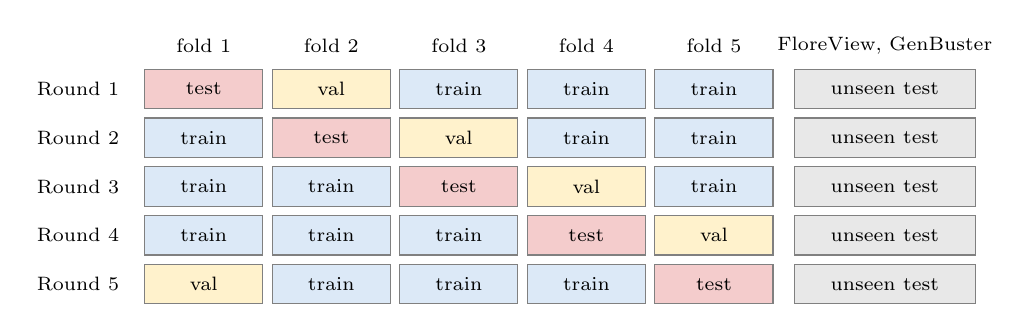
\begin{tikzpicture}[font=\scriptsize]
\foreach \r in {0,...,4} {
  \node[anchor=east] at (-0.2,-\r*0.62) {Round \the\numexpr\r+1\relax};
  \foreach \f in {0,...,4} {
    \pgfmathtruncatemacro{\v}{mod(\r+1,5)}
    \ifnum\f=\r \def\c{cOut}\def\t{test}\else\ifnum\f=\v \def\c{cEval}\def\t{val}\else\def\c{cPrep}\def\t{train}\fi\fi
    \node[draw=black!50, fill=\c, minimum width=1.5cm, minimum height=0.5cm] at (\f*1.62+0.75,-\r*0.62) {\t};
  }
  \node[draw=black!50, fill=cSrc, minimum width=2.3cm, minimum height=0.5cm] at (9.4,-\r*0.62) {unseen test};
}
\foreach \f in {0,...,4} \node at (\f*1.62+0.75,0.55) {fold \the\numexpr\f+1\relax};
\node at (9.4,0.55) {FloreView, GenBuster};
\end{tikzpicture}
\caption{5-fold cross-validation over camera-model groups. In each round one fold is the test set, the next fold is the
validation set (settings, early stopping, stacking) and the other three train the models. Every clip is tested exactly once,
always by a model that never saw its camera model.}\label{fig:folds}
\end{figure}

\subsection{Step 3 -- I-frame extraction (\texttt{03\_extract\_frames.py})}
\say{Turn every video into a small stack of comparable frames.}
Up to 30 I-frames per video (evenly spaced), converted to grey (luma) and centre-cropped to $480\times480$ in the sensor's own
orientation. Platform copies are rotated back and rescaled to the native geometry, so their pixels line up with the fingerprint.
\why{I-frames carry the most sensor noise; one common crop makes all videos comparable (two VISION phones record only
$640\times480$ or $800\times480$).}

\subsection{Step 4 -- PRNU fingerprints and baseline (\texttt{04\_prnu\_baseline.py})}
\say{Build each camera's fingerprint and measure how well the conventional PRNU method identifies cameras.}
A fingerprint $K$ per camera is estimated from its reference videos. Every sample video is correlated with every camera of its
dataset (PCE, PCE$_0$, NCC): the best-matching camera is the identification, and PCE$_0>60$ is the verification decision.

\begin{table}[H]\centering\small
\setlength{\tabcolsep}{5pt}\begin{tabular}{lrrrrr}\toprule
Dataset (cameras) & All cameras & Usable PRNU & Stabilised & False matches & EER \\\midrule
VISION (35) & 73.4\% & \textbf{100\%} (21) & 32\% (14) & 0\% & 0.0\%$^*$ \\
Video-ACID (44) & 59.1\% & \textbf{95.0\%} (25) & 12\% (19) & 0\% & 25.5\% \\
FloreView (45) & 26.2\% & \textbf{97.7\%} (10) & 7.5\% (35) & 0\% & 38.8\% \\\bottomrule
\end{tabular}\caption{Conventional PRNU attribution of genuine native videos (chance level $\approx$2--3\%). PRNU is close to
perfect when the phone keeps its PRNU and fails when electronic stabilisation removes it. $^*$non-stabilised cameras.}\label{tab:prnu}\end{table}

Processing also matters (VISION, non-stabilised phones): native 100\% $\rightarrow$ real YouTube copy 84.7\%
$\rightarrow$ real WhatsApp copy 60.7\%, and 0\% for WhatsApp copies of rotated (portrait) videos.
\why{this is the reference point for RQ2 and RQ3: it shows both the strength of PRNU and exactly where it breaks.}

\subsection{Step 5 -- The manipulated class: anti-forensic attacks (\texttt{05\_attacks.py})}
\say{Attack real videos the way a forger would, to create the ``manipulated'' class.}
Targets: 12 natural videos per camera (400 VISION videos; Phase 4 adds 528 Video-ACID videos). Each is decoded once, attacked,
and re-encoded with libx264 (one I-frame per second). With $Y$ the frame and $K$ a fingerprint scaled to a 1\% PRNU:
\begin{table}[H]\centering\small
\begin{tabularx}{\linewidth}{lYl}\toprule
Attack & What it does & Strengths \\\midrule
Removal & $Y' = Y - \alpha\,Y K_{\text{own}}$: subtracts the camera's own fingerprint & $\alpha$ = 0.25, 0.5, 1 \\
White-box removal & tunes $\alpha$ per clip on the analyst's own measurement until the correlation is $\approx$0 & per clip \\
Injection (transfer) & $Y' = Y + \alpha\,Y K_{\text{victim}}$: adds another camera's fingerprint; the clip claims the victim & $\alpha$ = 0.25, 0.5, 1 \\
Denoising & strong 3-D denoising (hqdn3d) that suppresses all sensor noise & 1$\times$, 2$\times$, 4$\times$ \\
Platform copies & WhatsApp-like (480 px, 0.110 bits/pixel, baseline profile) and YouTube-like (0.068 bits/pixel, high profile)
                  copies of the main attacks & -- \\
Genuine re-encodes & the same encoder without an attack (CRF 18, 20, 23, 28) + platform copies; label \emph{organic} & -- \\\bottomrule
\end{tabularx}\end{table}
\textbf{Realistic attacker.} The attacker never uses the analyst's reference videos: $K_{\text{own}}$ comes from the
\emph{other half} of the camera's natural videos, and $K_{\text{victim}}$ from a camera of another model in the same fold with a
usable PRNU. Example (Video-ACID camera M29\_DA): white-box removal leaves PCE$_0$ = 0.1; injection with $\alpha=1$ makes the
clip match the victim camera at PCE$_0$ = 1186 while the true camera remains faintly visible (61.5).
\why{genuine re-encodes through the same encoder are essential: without them the model could learn ``re-encoded = attacked''.}

\subsection{Step 6 -- The synthetic class: AI-generated video (\texttt{06\_synthetic.py})}
\say{Bring AI-generated videos into the same form as camera videos, and also forge camera fingerprints into them.}
\begin{itemize}
\item AI clips are re-encoded with the \emph{same} encoder, keyframe interval and crop as attacked and re-encoded clips, so
      the file format cannot reveal the class.
\item Each AI clip ``claims'' a random real camera from a random fold; its split follows that camera.
\item WhatsApp-like and YouTube-like copies of every AI clip.
\item \textbf{Khan-style PRNU transfer}: copies with a real camera's fingerprint injected ($\alpha$ = 0.5 and 1). A Sora clip
      injected with camera M29\_DA's fingerprint reaches PCE$_0$ = 376 / 1398, i.e.\ it passes conventional verification.
\item Phase 4 adds SVD, Mora, Text2Video-Zero and Pika. ModelScope ($256\times256$) and VideoCrafter2 ($512\times320$) were
      downloaded but \emph{not} used: they would need upscaling, and upscaling only AI clips would give the detector a shortcut.
\end{itemize}

\subsection{Step 7 / 7b -- Forensic features (\texttt{07\_features.py}, \texttt{07b\_noiseprint.py})}
\say{Measure, for every clip, everything that could separate genuine sensor noise from removed, forged or synthetic noise.}
\begin{table}[H]\centering\small
\begin{tabularx}{\linewidth}{lYl}\toprule
Group & Features & Level \\\midrule
PRNU & NCC and PCE$_0$ with the claimed camera; clip fingerprint scored against the claimed camera \emph{and the best other
       camera} (injection leaves the true camera's trace next to the victim's) & frame + clip \\
Residual & standard deviation, skewness, kurtosis of the noise residual & frame \\
FFT & spectral flatness, high-frequency share, peak ratio, periodic peaks, 8-pixel block energy & frame \\
TSNCS & correlation of consecutive residuals (temporal consistency) & frame \\
Noiseprint++ (7b) & statistics of the Noiseprint++ map; spectral similarity to the claimed camera & frame + clip \\\bottomrule
\end{tabularx}\caption{Feature groups: 18 per-frame features and 44 clip-level features (first 5 I-frames).}\end{table}

\subsection{Step 8 -- Models (\texttt{08\_models.py})}
\say{Train several classifiers on the features, and the conventional PCE rule as the baseline.}
\begin{itemize}
\item \textbf{Baseline}: PCE$_0$ with the claimed camera $> 60$ $\Rightarrow$ genuine (it cannot tell manipulated from synthetic).
\item \textbf{Classical}: SVM (RBF kernel) and XGBoost on the clip features; settings chosen on the validation cameras.
\item \textbf{Sequence models}: GRU, 1D-CNN and Transformer over the per-frame features, joined with the clip features
      (Adam, learning rate 0.001, L2 regularisation, class-balanced loss, early stopping on validation macro-F1).
\item Every clip contributes its first 5 I-frames; shorter clips repeat their own frames, so clip length is not a cue.
\item Two protocols: \emph{realistic} (all clips) and \emph{encoder-controlled} (only clips encoded by our pipeline, so
      encoder traces cannot separate the classes).
\end{itemize}

\subsection{Step 8b -- Vision Transformer (\texttt{08b\_vit.py}, \texttt{hvpf/vit.py})}
\say{A deep model that looks directly at the noise of the frames instead of hand-made features.}
ViT-S/16 pretrained on ImageNet-21k, fine-tuned on three SRM noise residuals of each I-frame (random $224\times224$ crops and
flips; AdamW, mixed precision, label smoothing, early stopping on validation macro-F1). A clip's prediction averages its
5 frames $\times$ 4 crops. Same input size as the base paper PDC-ViT. Phase 4 also runs it on 10 frames.

\subsection{Step 8c -- Fusion: calibration, ensembles, stacking, safe operating point (\texttt{08c\_ensemble.py})}
\say{Combine the models, using only validation cameras to decide how.}
\begin{itemize}
\item \textbf{Calibration}: shifts the class thresholds to maximise validation F1.
\item \textbf{Ensembles}: average the class probabilities of model groups (all models; the three best on validation; \dots).
\item \textbf{Stacking}: a logistic regression that learns from the validation predictions how much to trust each model.
      This is the best combination.
\item \textbf{Safe operating point} (Phase 4): the smallest shift towards ``genuine'' that accepts at least 95\% of genuine
      validation clips --- at most 5\% false accusations, the forensic priority.
\end{itemize}

\subsection{Step 9 -- Evaluation (\texttt{09\_evaluate.py})}
\say{Score every model the same way, on test cameras only.}
\begin{table}[H]\centering\small
\begin{tabularx}{\linewidth}{lYl}\toprule
Metric & What it measures & Used for \\\midrule
PVA & share of clips put in their true class (organic / manipulated / synthetic) & overall accuracy \\
Macro precision / recall / F1 & per class, then averaged with equal weight, so the smallest class counts as much as the largest & main ranking metric \\
AUC (genuine vs.\ not) & probability that a genuine clip scores higher than a fake; threshold-free & RQ3 (vs.\ PCE rule) \\
EER & error where false acceptance = false rejection & RQ3 \\
Detection rate per condition & share correct for each attack, strength, platform, generator, stabilisation & RQ2 \\
Macro-F1 drop & loss when one feature group is removed & RQ1 (ablation) \\
Compromise rate & share of injected clips accepted as genuine & Khan et al.\ comparison \\
Detection at fixed FPR & fakes caught while only 1/5/10\% of genuine clips are flagged & Bao et al.\ comparison \\\bottomrule
\end{tabularx}\end{table}
Results are the mean (and standard deviation) over the 5 folds; validation predictions are never counted.

\subsection{Step 10 -- Camera identification by training (\texttt{10\_camera\_id.py})}
\say{Answer ``which camera recorded this video?'' with a trained model, and combine it with PRNU.}
Per dataset, 80\% of each camera's recordings train a ViT with one output per camera; 20\% of its natural videos are test videos.
Versions of one recording and \emph{near-duplicate scenes} (thumbnail similarity $>0.9$, which wrongly merges only 0.2\% of
different VISION scenes) stay on one side of the split, so a test scene is never seen in training. The \textbf{hybrid} uses PRNU
when it is confident (PCE$_0$ above a threshold chosen on validation) and the ViT otherwise.

%=====================================================================================================
\section{Validity safeguards}\label{sec:validity}
\begin{table}[H]\centering\small
\begin{tabularx}{\linewidth}{lY}\toprule
Risk & Safeguard \\\midrule
Test camera seen in training & splits by camera model, across datasets; FloreView never in training \\
Fingerprint built from test videos & reference and sample videos are separate roles \\
Unrealistically strong attacker & attacker fingerprints from other videos than the analyst's references \\
\textbf{Shortcut 1: WhatsApp = genuine} (Phase 1) & WhatsApp-/YouTube-like copies of attacked and AI clips (Phase 2) \\
\textbf{Shortcut 2: clip length} & fixed 5-frame window; equal-length inputs (Phase 3); length-matched 5 vs.\ 10 frame test \\
\textbf{Shortcut 3: encoder traces} & genuine re-encodes through the same encoder; encoder-controlled protocol \\
Upscaled AI clips & only generators with native frames $\ge$ 480 pixels \\
Scene leakage (camera identification) & near-duplicate scene grouping (removes $\approx$4 points of inflation on FloreView) \\
Tuning on test data & all settings, calibration and stacking use validation cameras only \\\bottomrule
\end{tabularx}\end{table}

%=====================================================================================================
\section{Results so far}\label{sec:results}

\subsection{How the results evolved across phases}
\begin{table}[H]\centering\small
\setlength{\tabcolsep}{4.5pt}\begin{tabular}{lrlcccc}\toprule
Phase & Clips & Best model & Macro F1 & AUC & Controlled F1 & Unseen F1 \\\midrule
1 -- first full run & $\approx$8,000 & GRU & 0.852 & 0.930 & 0.703 & (AI only) \\
2 -- honest benchmark & 24,599 & XGBoost & 0.792 & 0.899 & 0.770 & 0.692 \\
3 -- ViT + stacking & 27,583 & Stacking & \textbf{0.851} & \textbf{0.941} & \textbf{0.816} & \textbf{0.863} \\
HVPF-2 (80/20 check) & 27,583 & Stacking & 0.850 & 0.941 & 0.818 & 0.893 \\
4 -- more data (running) & 46,799 & \multicolumn{5}{l}{\textit{results expected after the current run}} \\\bottomrule
\end{tabular}\caption{Best model per phase (realistic protocol, 5-fold cross-validation on unseen camera models, 5 frames).}
\label{tab:phases}\end{table}
\begin{itemize}
\item \textbf{Why Phase 2 is lower than Phase 1.} Phase 1 recognised 99\% of genuine WhatsApp copies only because every
      WhatsApp clip was genuine. After adding WhatsApp-like copies of fakes, that rate fell to 57\%: the earlier score was a
      shortcut, not skill. Phase 2 is the first honest benchmark.
\item \textbf{Phase 3 beats Phase 1 on equal terms.} On the clips all phases share, excluding the WhatsApp/YouTube copies,
      Phase 3 stacking reaches F1 0.796 / AUC 0.905 vs.\ 0.780 / 0.877 for Phase 1's best model.
\item \textbf{80/20 vs.\ 60/20/20} (HVPF-2): training on 80\% of the camera models changes single models by only +0.006 F1
      on average, smaller than the fold-to-fold spread. The conclusions do not depend on the split.
\end{itemize}

\subsection{Main results (Phase 3)}
\begin{table}[H]\centering\small
\begin{tabular}{lccccc}\toprule
Model & PVA & Macro F1 & AUC (3-class) & AUC genuine vs.\ not & EER \\\midrule
PCE rule (conventional) & -- & -- & -- & 0.549 & 0.449 \\
SVM & 0.765 & 0.769 $\pm$ 0.025 & 0.898 & 0.884 & 0.201 \\
XGBoost & 0.791 & 0.794 $\pm$ 0.029 & 0.927 & 0.913 & 0.177 \\
GRU & 0.773 & 0.779 $\pm$ 0.022 & 0.919 & 0.906 & 0.190 \\
1D-CNN & 0.768 & 0.774 $\pm$ 0.022 & 0.910 & 0.895 & 0.197 \\
Transformer & 0.770 & 0.780 $\pm$ 0.024 & 0.916 & 0.902 & 0.194 \\
ViT (noise residuals) & 0.806 & 0.820 $\pm$ 0.017 & 0.933 & 0.912 & 0.182 \\
Ensemble (all models) & 0.807 & 0.814 $\pm$ 0.022 & 0.941 & 0.927 & 0.167 \\
\textbf{Stacking} & \textbf{0.836} & \textbf{0.851 $\pm$ 0.014} & \textbf{0.955} & \textbf{0.941} & \textbf{0.149} \\\bottomrule
\end{tabular}\caption{Realistic protocol, 5-fold cross-validation, test camera models never seen in training (27,583 clips).
Encoder-controlled protocol: stacking 0.816 F1, AUC 0.906 (PCE rule 0.513).}\label{tab:main}\end{table}

\subsection{RQ1 -- Which characteristics separate organic from synthetic or manipulated noise?}\label{sec:rq1}
\begin{table}[H]\centering\small
\begin{tabular}{lccccc}\toprule
Removed feature group & SVM & XGBoost & GRU & 1D-CNN & Transformer \\\midrule
Noiseprint++ statistics & 0.053 & 0.054 & 0.052 & 0.048 & 0.067 \\
TSNCS (temporal consistency) & 0.016 & 0.029 & 0.013 & 0.015 & 0.013 \\
PRNU & 0.006 & 0.023 & 0.015 & 0.005 & 0.014 \\
Residual statistics & 0.001 & 0.004 & 0.005 & $-0.001$ & 0.004 \\
FFT statistics & 0.001 & $-0.001$ & $-0.006$ & 0.003 & 0.005 \\\bottomrule
\end{tabular}\caption{Drop in macro F1 when one feature group is removed (realistic, 5-fold). Larger = more important.}\end{table}
\textbf{Answer:} the most discriminative evidence is the camera-model-level noise structure (Noiseprint++), followed by
\emph{temporal} noise consistency and the PRNU match itself (including the ``best other camera'' score that exposes
injection). Simple residual and frequency statistics add almost nothing once these are present. The ViT, which learns from the
raw noise residual, is the best single model, so learned noise representations add information beyond hand-made features.

\subsection{RQ2 -- How does processing affect PRNU and noise-based analysis?}\label{sec:rq2}
\begin{itemize}
\item \textbf{Platform re-compression} is the strongest effect: PRNU identification falls from 100\% (native) to 84.7\%
      (YouTube) and 60.7\% (WhatsApp); 0\% for rotated WhatsApp copies. For the detector, genuine WhatsApp copies are
      recognised only 48\% of the time (stacking): heavy compression erases the evidence that separates genuine from attacked.
\item \textbf{Electronic stabilisation} destroys the PRNU (identification 7--32\% for stabilised phones vs.\ 95--100\% otherwise).
\item \textbf{Attack strength}: stacking detects removal at $\alpha$ = 0.25 / 1 in 63\% / 98\% of clips and injection at
      $\alpha$ = 0.25 / 1 in 72\% / 93\%. The PCE rule ``detects'' removal (low PCE) but is fooled by injection: only 2\% of
      full-strength injections are rejected.
\item \textbf{Compression of AI clips}: after WhatsApp-like compression, AI clips from CogVideo, Kling and OpenSora are still
      caught 98--99\% of the time, Sora 57\% (only 51 clips), and unseen generators 42\%.
\end{itemize}

\subsection{RQ3 -- Does the hybrid framework beat the conventional method?}\label{sec:rq3}
\begin{table}[H]\centering\small
\begin{tabularx}{\linewidth}{Ycc>{\raggedright\arraybackslash}p{3.3cm}}\toprule
 & PCE rule & Hybrid (stacking) & Reference \\\midrule
AUC genuine vs.\ not (5-fold) & 0.549 & \textbf{0.941} & \\
EER & 0.449 & \textbf{0.149} & \\
Fakes caught at 1\% false positives & 5.3\% & \textbf{56.4\%} & Bao et al.\ 2024 (ROC only) \\
Camera-to-camera injection accepted ($\alpha=1$) & 98\% & \textbf{1\%} & Khan et al.\ 2025: 85.5\% (images) \\
AI video + injected PRNU accepted ($\alpha=1$), seen generators & 98\% & \textbf{0\%} & \\
AI video + injected PRNU accepted ($\alpha=1$), unseen generators & 96\% & \textbf{1\%} & \\\bottomrule
\end{tabularx}\caption{Hybrid vs.\ conventional PRNU verification (Phase 3).}\end{table}
\textbf{Answer: yes.} The conventional rule is fooled by exactly the attack this thesis targets (fingerprint injection,
including into AI video), while the hybrid framework catches it. Of the injected AI clips, 99\% are recognised as AI-made: the
injection makes the clip match the camera, but it does not remove the other traces the models use.

\subsection{Unseen sources}
Models trained on VISION + ACID + GenVidBench were tested on FloreView (new phones) and GenBuster (new generators). Stacking
reaches F1 0.863 and AUC 0.965. The ViT is the most robust single model: it recognises 90\% of FloreView genuine videos
(XGBoost 55\%), including 88\% of stabilised phones without a usable PRNU.

\subsection{Camera identification by training (Step 10, Phase 4)}
\begin{table}[H]\centering\small
\setlength{\tabcolsep}{4.5pt}\begin{tabular}{lrrrrr}\toprule
Test videos (cameras) & Trained ViT & PRNU & \textbf{Hybrid} & ViT: model right & PDC-ViT$^\dagger$ \\\midrule
VISION (35) & 49.7\% & 55.9\% & \textbf{67.4\%} & 56.2\% & 94.3\% \\
Video-ACID (44) & 90.9\% & 57.5\% & \textbf{94.9\%} & 99.5\% & 74.77\% \\
FloreView (45) & 89.0\% & 25.9\% & \textbf{90.1\%} & 89.0\% & -- \\\midrule
Stabilised: ACID / FloreView & 89.7 / 86.8\% & 11.8 / 6.8\% & 90.2 / 87.5\% & & \\\bottomrule
\end{tabular}\caption{Closed-set camera identification (80/20 per camera, scene-grouped). The hybrid uses PRNU when it is
confident and the ViT otherwise. $^\dagger$as reported in the paper (Video-ACID there: 26 cameras + WhatsApp copies).}\label{tab:camid}\end{table}
The two methods complement each other: the ViT almost always finds the right camera \emph{model} (99.5\% on ACID) and keeps
working on stabilised phones, while PRNU separates individual devices of the same model. VISION is hardest for the ViT
(about 30 training videos per camera, strict scene split, WhatsApp/YouTube copies in the test set).

\subsection{Comparison with the base papers}
\begin{table}[H]\centering\small
\begin{tabularx}{\linewidth}{lYY}\toprule
Base paper & What it reports & HVPF \\\midrule
PDC-ViT (Elharrouss et al.\ 2025) & camera identification: VISION 94.3\%, Video-ACID 74.77\%; clean data only, every camera in
   training & PRNU 100\% / 95\% on non-stabilised cameras; trained hybrid 94.9\% on Video-ACID (67.4\% on VISION with a stricter
   scene split); tested under attack \\
Khan et al.\ 2025 & PRNU transfer fools verification for 85.5\% of images (incl.\ AI images) & same attack on video: PCE rule
   fooled 96--98\%, hybrid 0--1\% \\
Bao et al.\ 2024 & frame-deletion detection from inter-frame noise; ROC curves, focus on low false-positive rates &
   56.4\% of fakes caught at 1\% false positives (PCE rule 5.3\%) \\\bottomrule
\end{tabularx}\end{table}

%=====================================================================================================
\section{Current work: Phase 4}\label{sec:phase4}
Phase 4 addresses the weak spots found in Phase 3:
\begin{table}[H]\centering\small
\begin{tabularx}{\linewidth}{lYl}\toprule
Weak spot & Change & Status \\\midrule
Manipulated class from 35 VISION cameras only & all attacks also on 528 Video-ACID videos (9,504 clips; 79 cameras) & done \\
Genuine re-shared clips called ``manipulated'' & 3,712 more genuine platform copies; safe operating point & done / running \\
Unseen generators after WhatsApp (42\%) & four more training generators (SVD, Mora, Text2Video-Zero, Pika; 6,000 clips) & done \\
Single-frame ViT & ViT also with 10 frames & running \\
Scene leakage in camera identification & near-duplicate scene grouping & done \\\bottomrule
\end{tabularx}\end{table}
Feature extraction, all models, the ViT and evaluation are running (about 14 hours). A first test of the safe operating point
on Phase 3 predictions shows the trade-off it must manage: genuine clips accepted rises from 79\% to 95\%, AI clips caught stays
at 97\%, but caught attacks fall from 82\% to 53\%. The additional genuine platform copies are meant to reduce this overlap.

%=====================================================================================================
\section{Limitations and threats to validity}
\begin{itemize}
\item \textbf{Attack implementation}: all attacks are our own implementation; an attacker who knows the detector (adaptive
      attack) is not yet evaluated.
\item \textbf{Simulated platforms}: platform copies of fakes are simulated; only genuine VISION videos have real WhatsApp and
      YouTube copies.
\item \textbf{Genuine vs.\ attacked after heavy compression}: the main source of false accusations (genuine re-encoded
      WhatsApp-like copies).
\item \textbf{Generators}: Sora has only 51 clips; AI video evolves quickly.
\item \textbf{Baselines}: PDC-ViT numbers are taken from the paper; it has not yet been re-run on our splits.
\end{itemize}

\section{Plan until the final evaluation}
\begin{enumerate}
\item Finish Phase 4 and report its results against Phase 3 (in progress).
\item Re-run a PDC-ViT-style model and one published AI-video detector on our own splits (same-protocol baselines).
\item One adaptive attack aimed at the detector, or a clearly bounded threat model.
\item A small real-upload test: genuine and fake clips through real WhatsApp and YouTube.
\item Significance tests and confidence intervals for the main comparisons.
\item Thesis chapters (methodology, results, discussion) and a focused paper on PRNU transfer attacks on video.
\end{enumerate}

%=====================================================================================================
\appendix
\section{Likely panel questions}
\begin{description}[leftmargin=0pt]
\item[Why split by camera model and not randomly?] A random split puts videos of the same phone in training and test; the
      model then recognises the phone instead of learning what genuine noise looks like. Model-level grouping is stricter.
\item[Why are the Phase 2 scores lower than Phase 1?] Phase 1 contained a shortcut (all WhatsApp clips were genuine). Phase 2
      removed it; lower but honest scores are the correct baseline. Phase 3 then exceeded Phase 1 on equal terms.
\item[How do you know the model is not just recognising your encoder?] Genuine clips go through the same encoder, and the
      encoder-controlled protocol uses only our own encoded clips: stacking still reaches F1 0.816 there.
\item[Is PRNU still needed if the ViT is better?] Yes. PRNU separates individual devices of the same model and verifies a
      specific camera; the hybrid is best in every setting, and the PRNU ``best other camera'' score exposes injection.
\item[Why not use the low-resolution AI generators?] They would need upscaling. If only AI clips were upscaled, the detector
      could learn ``upscaled = AI'', which is useless against modern full-resolution generators.
\item[Why I-frames only?] They are complete frames with the most sensor noise; predicted frames are dominated by compression.
\item[Is the 80/20 split better?] It was tested (HVPF-2): +0.006 F1 on average for single models, within the fold-to-fold
      variation. The main protocol (60/20/20 + 5 folds) keeps a clean validation set for every decision.
\item[What happens with real WhatsApp?] For genuine VISION videos with real WhatsApp copies the detector recognises 48\%; this is
      the main open problem and the focus of Phase 4.
\end{description}

\section{Glossary}
\begin{description}[leftmargin=0pt, itemsep=1pt]
\item[PRNU] photo-response non-uniformity; the sensor fingerprint.
\item[PCE / PCE$_0$] peak-to-correlation energy; the conventional fingerprint match score (threshold 60).
\item[Organic / manipulated / synthetic] genuine camera video / anti-forensic attack on the fingerprint / AI-generated video.
\item[PVA] provenance verification accuracy: share of clips assigned to their true class.
\item[Macro F1] F1 per class, averaged with equal weight.
\item[AUC / EER] threshold-free separability / error where false acceptance equals false rejection.
\item[Stacking] a model that learns how to combine other models' predictions.
\item[Closed set / open set] all test cameras seen in training (camera identification) / test cameras unseen (provenance).
\end{description}

\section{Reproducibility}
Code: \url{https://github.com/TalhaAslam44/PRNU-Research} (branch \texttt{main}; the 80/20 study on branch \texttt{hvpf-2}).
Every step is a script in \texttt{scripts/} (01--10) with a VS Code task; \texttt{scripts/run\_phase4.sh} runs the current
phase. Detailed results: \texttt{report/results\_phase3.pdf} (Phase 3) and \texttt{results\_hvpf2.pdf} (HVPF-2 branch).

\begin{thebibliography}{9}
\bibitem{pdcvit} O.~Elharrouss et al., ``PDC-ViT: source camera identification using pixel difference convolution and vision
  transformer,'' \emph{Neural Computing and Applications}, 2025, doi:10.1007/s00521-025-11004-z.
\bibitem{khan2025} Khan, Hasan, Islam, ``Spoofing camera source attribution via PRNU transfer attacks,'' \emph{ISC 2025},
  Springer LNCS 16186, pp.~279--299, 2025.
\bibitem{bao2024} Bao et al., ``Anti-forensics video forgery detection via noise transfer matrix,'' \emph{Sensors} 24(16):5341, 2024.
\bibitem{vision} D.~Shullani et al., ``VISION: a video and image dataset for source identification,'' \emph{EURASIP J.\ on
  Information Security}, 2017.
\bibitem{trufor} F.~Guillaro et al., ``TruFor: leveraging all-round clues for trustworthy image forgery detection and
  localization,'' \emph{CVPR}, 2023 (Noiseprint++).
\end{thebibliography}
\end{document}
